\documentclass[10pt,a4paper]{article}
\usepackage[utf8]{inputenc}
\usepackage[german]{babel}
\usepackage{mathrsfs}
\usepackage{amsmath}
\usepackage{amsfonts}
\usepackage{amssymb}
\usepackage{amsthm}
\usepackage{graphicx}
\usepackage{float}
\usepackage[left=2cm,right=2cm,top=2cm,bottom=2cm]{geometry}

\begin{document}

\section{Aufgabe 17}
Wenn $n \in \mathbb{N}_{0}$ 0 ist, ist $g_{0}$ die Nullfunktion, die ich nicht zeichne.
\begin{figure}[H]
  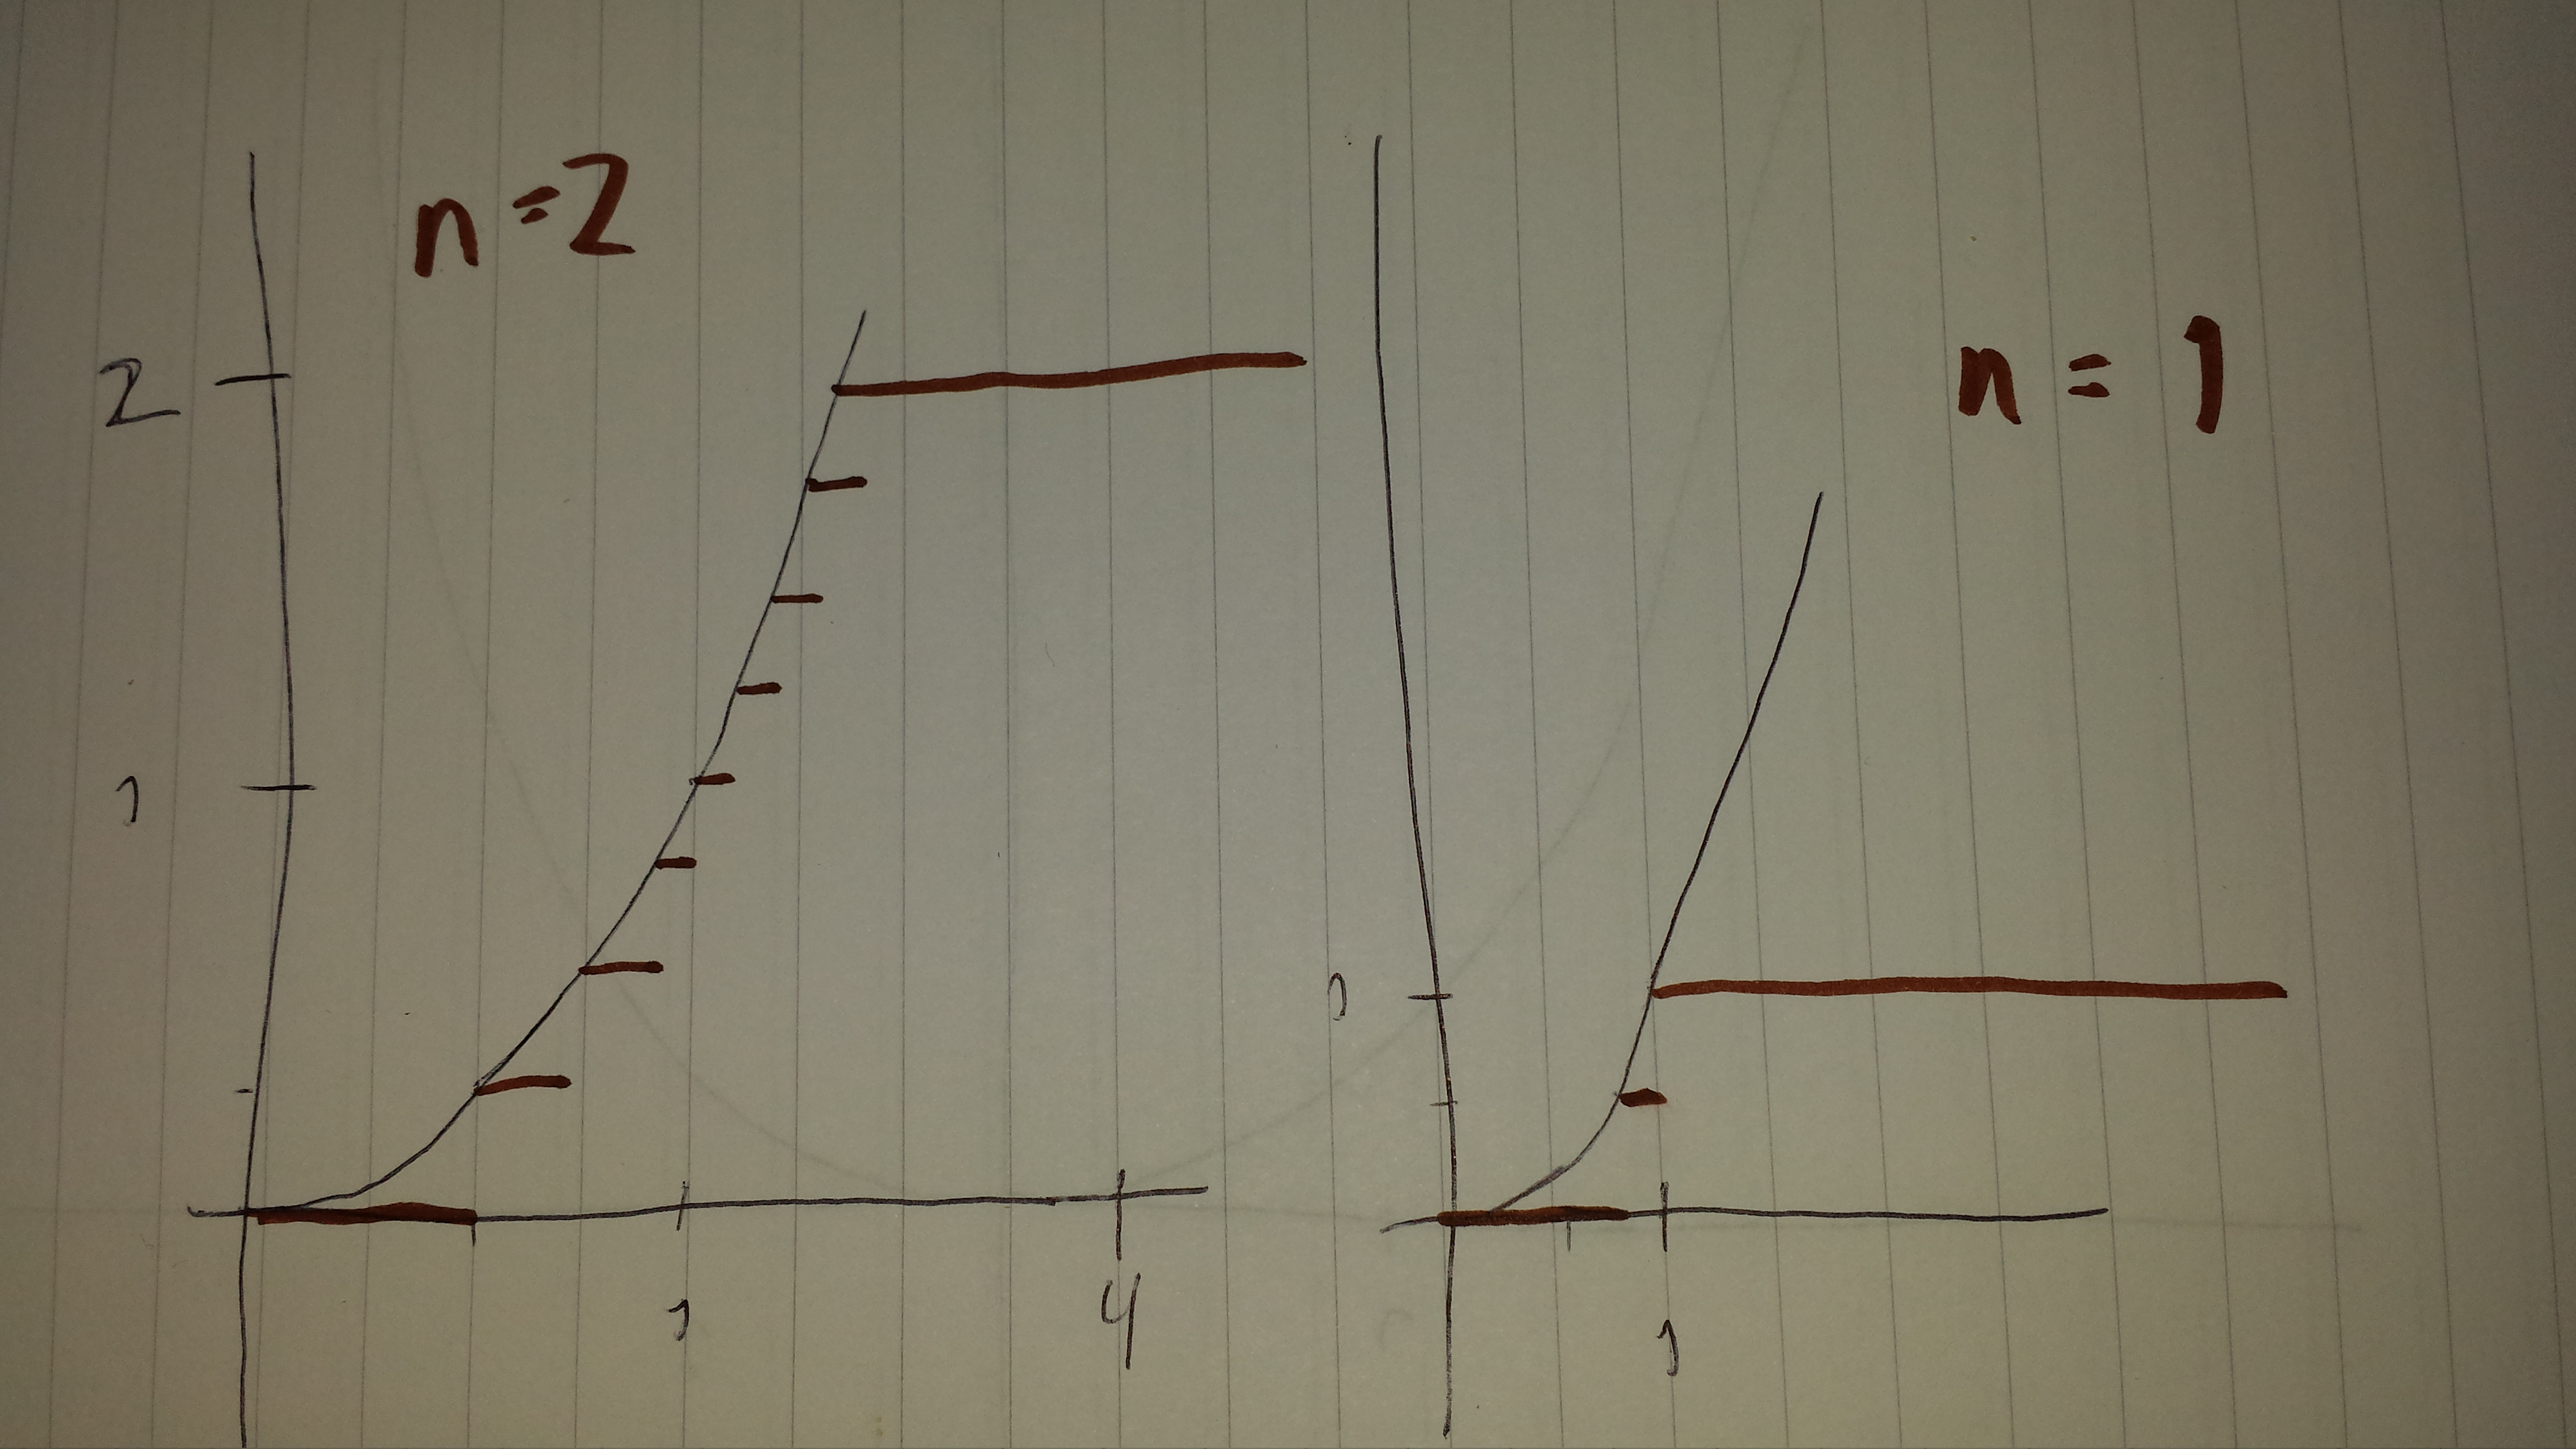
\includegraphics[width=400pt]{5_1}
\end{figure}
Auf den Zeichnungen habe ich es nicht so gut hinbekommen, aber die Stufen werden immer kürzer (außer der letzten).
Und ich habe hier nur die positive Hälfte gezeichnet.
Eigentlich ist es natürlich an der Y-Achse gespiegelt.

\section{Aufgabe 18}

\subsection{Teil a}

\subsection{Teil b}

\subsection{Teil c}
\begin{proof}
  $\Rightarrow$: Sei $lim_{n \rightarrow \infty} a_{n} = a$.
  Nach Definition gibt es für jedes $\epsilon$ ein $n$, sodass $|a_{k} - a| < \frac{\epsilon}{2} \Leftrightarrow -\frac{\epsilon}{2} < a_{k} - a < \frac{\epsilon}{2}$ für alle $k \ge n$.
  Dann ist
  \begin{align*}
    & a - \epsilon < \inf \{ a_{k} \mid k \ge n \} \le \sup \{ a_{k} \mid k \ge n \} < a + \epsilon\\
    \Leftrightarrow & -\epsilon < \inf \{ a_{k} \mid k \ge n \} - a \le \sup \{ a_{k} \mid k \ge n \} - a < \epsilon\\
    \Leftrightarrow & -\epsilon < \inf \{ a_{k} \mid k \ge n \} - a \le \sup \{ a_{k} \mid k \ge n \} - a < \epsilon\\
    \Leftrightarrow & |\inf \{ a_{k} \mid k \ge n \} - a| < \epsilon\ \land\ |\sup \{ a_{k} \mid k \ge n \} - a| < \epsilon\\
    \Leftrightarrow & \liminf_{n \rightarrow \infty} a_{n} = a = \limsup_{n \rightarrow \infty} a_{n}
  \end{align*}
  Die andere Richtung ist einfach rückwärts.
\end{proof}

\subsection{Teil d}

\section{Aufgabe 19}

\section{Aufgabe 20}

\section{Aufgabe 21}
\begin{equation}
  f_{n}(x) = 
  \begin{cases}
    & 1\textit{ wenn $n \le x \le n + 1$}\\
    & 0\textit{ sonst}
  \end{cases}
\end{equation}
\begin{equation}
  g_{n}(x) = 
  \begin{cases}
    & 2\textit{ wenn $n \le x \le n + 1$}\\
    & 0\textit{ sonst}
  \end{cases}
\end{equation}
Dann konvergieren bei Folgen gegen die $0$-Funktion, weil es für jedes $x$ ein $N$ gibt, sodass $f_{n}(x) = g_{n}(x) = 0$ für alle $n \ge N$.
Allerdings ist $\lim_{n \rightarrow \infty} \int f_{n} d \lambda^{1} = 1$ und $\lim_{n \rightarrow \infty} \int g_{n} d \lambda^{1} = 2$.

\end{document}